\documentclass[11pt,xcolor=dvipsnames]{beamer}
\usepackage{pdfpages}
\usepackage{verbatim}
\usepackage{amssymb}
\usepackage{amsmath}
\usepackage{amsfonts}
\usepackage[T1]{fontenc}
\usepackage{lmodern}
\usepackage{verbatim} 	% required for multiline comments using \begin{comment}
\usepackage{ragged2e}   % this is used to justify any type of text
\usetheme[hideothersubsections,width=22mm]{Hannover}
\usecolortheme{sidebartab,beaver}
\setbeamercolor{section in sidebar}{fg=MidnightBlue,bg=white}
\setbeamercolor{section in sidebar shaded}{fg=CadetBlue}
\setbeamercolor{subsection in sidebar}{fg=MidnightBlue,bg=white}
\setbeamercolor{subsection in sidebar shaded}{fg=CadetBlue}
\setbeamercolor{title in sidebar}{fg=black}
\setbeamercolor{author in sidebar}{fg=ForestGreen}
\title{Support Vector Machine Approach to Automated Cardiac SPECT diagnosis}
% \author{Varun B Patil}		
%\author{8th Semester Project Presentation \\[1cm]Varun B Patil \\[1.2cm]}
\author[]{8th Semester Project Presentation \\[1cm]Varun B Patil \\[1.2cm]}
% if u dont want author to appear in sidebar write author[]{Varun B Patil}

% \institute{Sri Jayachamarajendra College of Engineering, Mysore}
% \date{2012}
\date{2012 \small \\[0.2cm]Dept. of Computer Science \& Engineering \\[0.2cm]Sri Jayachamarajendra College of Engineering, Mysore}

\renewcommand{\raggedright}{\leftskip=0pt \rightskip=4pt}  
% this is required to justify text in beamer class
% but this one only justifies text with \item{}														   
														   

\begin{comment}
\AtBeginSection[]
{
  \begin{frame}
    \frametitle{Table of Contents}
    \tableofcontents[currentsection]
  \end{frame}
}

\AtBeginSubsection[]
{
  \begin{frame}
    \frametitle{Table of Contents}
    \tableofcontents[currentsection,currentsubsection]
  \end{frame}
}
\end{comment}



\begin{document}


\begingroup	% limits the effect of a change
\makeatletter	% makeatletter and makeatother are required to access 
                % \beamer@sidebarwidth
\setlength{\hoffset}{-.5\beamer@sidebarwidth}	% required to center the title page
\makeatother
\begin{frame}[plain]	% "plain" removes the sidebar from this slide alone
\titlepage
\end{frame}
\endgroup

\setbeamercolor{background canvas}{bg=}

\includepdf[scale=1.7]{title_page.pdf}


\begin{comment}
%=================================================================================
\section{Introduction}	% this is what comes at the side of the slide
% sections and subsections should come outside the frame environment
\begin{frame}
\frametitle{What is SPECT ?}			% this is the heading that gets
						% displayed within the slide

\justifying
SPECT stands for {\color{PineGreen}Single Photon Emission Computerized Tomography}. It is the state-of-the-art in detecting various types of cardiac diseases. SPECT provides us with computer images which can be analyzed to determine the type of cardiac disease. The aim of this project is to make sense out of the data produced after processing these SPECT images.\\
\end{frame}
%=================================================================================





%=================================================================================
%\section{What is SVM?}		% even this frame is made to come under the same section as above frame	
\begin{frame}
\frametitle{What is SVM ?}	
\justifying
SVM stands for {\color{PineGreen}Support Vector Machines}. It is a supervised machine learning algorithm which we use here to classify instances of SPECT data as indicating possible cardiac disease or not. SVM learns from pre-classified data we provide and then automatically classifies un-classified data based on rules learned previously. \\
\end{frame}
%=================================================================================


%=================================================================================
\section{SPECT images}	
\begin{frame}
\frametitle{Some SPECT images \ldots}	
\centering
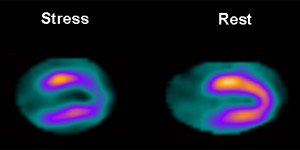
\includegraphics[scale=1]{spect_images.png}
\end{frame}
%=================================================================================




%=================================================================================
\section{Inputs}	
\begin{frame}
\frametitle{Inputs to program}	
\begin{itemize}
\item SPECT is actually images. It has to be preprocessed to generate numerical data that the program can work on.\\
\item SPECT images are few and far between. For all computational machine learning purposes, UCI maintains a comprehensive database of numerical SPECT data collected from some of the best medical institutions around the world that we will be using.\\ 		
\item The data set we will be using was obtained from {\color{PineGreen} \\ \small http://archive.ics.uci.edu/ml/datasets/SPECT+Heart}
\end{itemize}
\end{frame}
%=================================================================================


%=================================================================================
\begin{frame}
\frametitle{Structure of input data}	
\begin{itemize}
\item The UCI data set is a comma-seperated-value file (CSV) which we read into the octave program as a two dimensional matrix using a built in function called csvread(). \\
\item There are binary values for about 23 features indicating the presence or absence of a particular feature in that particular SPECT image instance. These features include left ventricular ejection fraction, stroke volume, myocardial perfusion, etc. \\
\item The data is provided in two parts: {\color{PineGreen}Training set} used to train the machine learning classifier and {\color{PineGreen}Test set} used to test the classifier's accuracy.
\end{itemize}
\end{frame}
%=================================================================================



%=================================================================================
\begin{frame}
\frametitle{Dividing the Test Set}	
\begin{itemize}
\item The Test Set itself is further divided into a {\color{PineGreen}Cross Validation set} and a {\color{PineGreen}Test set}. The CV consists of random samples from the Test Set. \\
\item The cross validation(CV) set is primarily used to tune the classifier program for best performance; it is not used to gauge the accuracy of the classifier. For example, the CV set is used to select the best possible values for C and sigma used in the SVM algorithm.\\
\item The remaining part of the Test Set is the one that is actually used to measure the accuracy of the classifier after it has been trained on the Training Set.
\end{itemize}
\end{frame}
%=================================================================================


%=================================================================================
\begin{frame}
\frametitle{Dividing the Test Set}	
\begin{itemize}
\item Usually the data is divided as training set(60\%), CV set(20\%) and test set(20\%). The distribution between the sets is done randomly. Then, the hypothesis that minimizes the CV set error(fraction of CV set instances that are wrongly classified) is chosen and the error on the test set is reported as the generalized error.
\end{itemize}
\end{frame}
%=================================================================================
\end{comment}


%=================================================================================
\section{Algorithm}	
\begin{frame}
\frametitle{SVM algorithm}	
\begin{itemize}
\item The SVM machine learning algorithm aims to find the best relationship between the features and its class so as to minimize the error in classification.\\ 
\item The algorithm we employ is called {\color{PineGreen}SMO(Sequential Minimal Optimization)} and it finds the best possible class to which a particular instance of SPECT data belongs to. The term ``best class" here means the class which minimizes the classification error or likewise improves the classification accuracy.\\
\item The two classes possible for any SPECT instance are: indicates possible cardiac disease, does not indicate cardiac disease(future enhancements to the project will include more fine grained classification or multiclass classification).
w SVM works for non-linear decision boundaries:\\
\end{itemize}
\end{frame}
%=================================================================================


%=================================================================================
\begin{frame}
\frametitle{Choices in implementation}	
\begin{itemize}
\item The SVM algorithm we have implemented can either use a {\color{PineGreen}Linear Kernel} or a {\color{PineGreen}Gaussian Kernel}. \\
\item A {\color{PineGreen}Linear Kernel} can be imagined to be a {\color{PineGreen}straight-line seperation} between the classes(or a planar seperation in the case of multidimensional data).\\
\item The {\color{PineGreen}Gaussian Kernel} on the other hand can be visualized as a {\color{PineGreen}non-linear seperation} between classes which also means a non-planar or curved seperation between classes of multidimensional data.
\end{itemize}
\medskip
\begin{displaymath}K_{linear}(x^i, x^j) = x^i * x^j\end{displaymath}
\begin{displaymath}K_{gaussian}(x^i, x^j) = \exp(-\frac{||x^i - x^j||^2}{2\sigma^2})\end{displaymath}
\end{frame}
%=================================================================================


%=================================================================================
\begin{frame}
\frametitle{Linear Vs. Gaussian}
\begin{block}{Which one do you use ?}
\begin{itemize}
\item With choice comes the problem of deciding which one to use for the particular problem at hand.\\
\item A Linear Kernel is usually employed when the number of features is more than the number of samples and a Gaussian Kernel is employed when the number of samples is more than the number of features.\\
\item And also, the kernel used depends on whether the data itself is linearly-seperable or not.
\end{itemize}
\end{block}	
\end{frame}
%=================================================================================




%=================================================================================
\begin{frame}
\frametitle{Linear Vs. Gaussian}
\centering
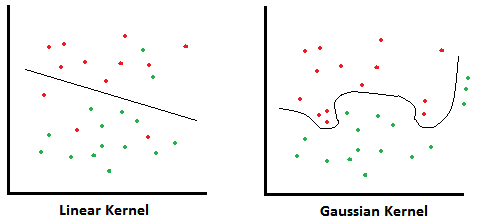
\includegraphics[scale=0.72]{linear_gaussian.png}
\end{frame}
%=================================================================================


%=================================================================================
\begin{frame}
\frametitle{Cost Function}
The cost function in SVM is:
\begin{displaymath}
\sum_{i=1}^{m}(y^i * cost_{1}(z)  +  (1-y^i) * cost_{0}(z)) + (\frac{\lambda}{2} * \sum_{i=1}^{m}(\Theta_{i}^2))
\end{displaymath}
\smallskip
where $z = \Theta^T x$
\smallskip
\begin{itemize}
\item $cost_1()$ graph has 0 value for $z>=1$ and a straight line for $z<1$\\
\item $cost_0()$ graph has 0 value for $z<=-1$ and a straight line for $z>-1$\\
\end{itemize}
\medskip
So, to minimize cost function, we want z to be $>=1$ when the class is 1 and we want z to be $<=-1$ when the class is 0.
\end{frame}
%=================================================================================





%=================================================================================
\begin{frame}
\frametitle{Optimization}
By convention, we optimize:\\
\begin{displaymath}J = (C * A) + B\end{displaymath}
\medskip
where\\
\medskip        
\begin{displaymath}A = \Sigma(y^i * cost_{1}(z)  +  (1-y^i) * cost_{0}(z))\end{displaymath}    
\begin{displaymath}B = \frac{1}{2} \Sigma(\Theta^2)\end{displaymath}
\begin{displaymath}cost_{1}(z) \approx -\log(z)\end{displaymath}
\begin{displaymath}cost_{0}(z) \approx -\log(1 - z)\end{displaymath}
\end{frame}
%=================================================================================


%=================================================================================
\begin{frame}
\frametitle{Optimization}
\begin{itemize}
\item We see that the definitions for $cost_0()$ and $cost_1()$ above are nothing but straight line approximations to the logarithmic curves. This is done in order to reduce execution time.\\
\item By minimizing the above equation $J = C*A + B$, we learn the optimal parameters $\Theta$\\
\item Once we know $\Theta$, we can predict the class as follows: \\
\begin{displaymath}if(\Theta^Tx) >= 0, \text{predict class} = 1\end{displaymath}
\begin{displaymath}if(\Theta^Tx) <= 0, \text{predict class} = 0\end{displaymath}
\end{itemize}
\end{frame}
%=================================================================================


%=================================================================================
\begin{frame}
\frametitle{Role of C and $\sigma$}
\begin{itemize}
\item We noted earlier that C and $\sigma$ are two important parameters that need to be decided by examining the Cross Validation set.\\
\item  Informally, the C parameter is a positive value that controls the penalty for misclassified training examples. A large C parameter tells the SVM to try to classify all the examples correctly(large margin). However, large C means that it is more susceptible to outliers and does not give a natural fit for the data.
\end{itemize}
\end{frame}
%=================================================================================


%=================================================================================
\begin{frame}
\frametitle{Role of C and $\sigma$}
\begin{itemize}
\item SVM's are large margin classifiers meaning that the seperation between classes in maximum. In other words, the distance of the seperating boundary from the nearest data point is large. Such a large margin SVM classifier is obtained by setting C to a large value.\\
\item A large value for C value means that the term A should be made close to 0 to make J less. In other words, if C is made large, then we only need to optimize $\frac{1}{2}\Sigma(\Theta^2)$\\
\item The only problem is that large C means greater susceptibility to outliers. So we have no choice but to make C small.    
\end{itemize}
\end{frame}
%=================================================================================


%=================================================================================
\begin{frame}
\frametitle{Role of C and $\sigma$}
\begin{itemize}
\item $\sigma$ is a parameter of the Gaussian Kernel which determines how fast the ``similarity measure" approaches 0 for data points that are further apart. If $\sigma$ is large, the similarity changes slowly and can cause underfitting. If $\sigma$ is small, the similarity changes fast and can cause overfitting.\\
\item In practice, C and $\sigma$ are selected from a set of highly possible values for both C and $\sigma$ where the values vary approximately by a factor of 10, by testing all possible combinations of C and $\sigma$ for the one that gives the least error in classification of the CV set. In our implementation, the values of C and $\sigma$ take on the following set of values
\begin{displaymath}C = [0.01, 0.03, 0.1, 0.3, 1, 3, 10, 30]\end{displaymath}
\begin{displaymath}\sigma = [0.01, 0.03, 0.1, 0.3, 1, 3, 10, 30]\end{displaymath}
\end{itemize}
\end{frame}
%=================================================================================


%=================================================================================
\begin{frame}
\frametitle{Non-linear decision boundaries}
How SVM works for non-linear decision boundaries:\\
\begin{itemize}
\item Pick landmarks $l_1$, $l_2$,...(usually these are nothing but the data points themselves).\\
\item Now the similarity(or kernel) function = $\exp(-\frac{||x - l_i||^2}{2\sigma^2})$
\item The hypothesis here is $\Theta_1*f_1$ + $\Theta_2*f_2$ + $\Theta_3*f_3$ + .....\\
\item $f_1$ is called the similarity of the data points to the landmark 1 (i.e, $l_1$) and so on.\\
\item When the data point is very close to the landmark, we get the corrseponding feature almost equal to 1. When the data point is very far from the landmark, we get the corrseponding feature almost equal to 0. That is, as the data point moves farther from the landmark, the value of feature decreases.
\end{itemize}
\end{frame}
%=================================================================================



%=================================================================================
\begin{frame}
\frametitle{Non-linear decision boundaries}
\begin{itemize}
\item How fast the feature value decreases depends on the $\sigma$ for gaussian kernels.\\
\item If $\sigma$ is large, the feature value decreases slowly as the data point moves away from the landmark. This is called high bias or lower variance(underfitting).\\
\item If $\sigma$ is small, the feature value decreases fast as the data point moves away from the landmark. This is called high variance or lower bias(overfitting).
\item Using the kernals approach, the cost function is also changed. Instead of $z = \Theta^T x$, we use $z = \Theta^T f$
\end{itemize}
\end{frame}
%=================================================================================



\begin{comment}
%=================================================================================
\section{Output}	
\begin{frame}
\frametitle{Expectations from the algorithm}
\begin{itemize}
\item When all is said and done, you expect the classifier to tell you the class to which a particular SPECT instance belongs to. One way to check whether what the classifier predicts is ``upto the mark" is to compare the result with already known values.\\
\item There are several ways to gauge this ``upto mark" notion in terms of numerical values.\\
\item {\color{PineGreen}Prediction Accuracy} is the fraction of the instances in the Test set that are correctly classified.\\
\begin{displaymath}\text{Accuracy} = \frac{\text{Test set instances correctly classified}}{\text{total Test set instances}}\end{displaymath}    
\end{itemize}
\end{frame}
%=================================================================================



%=================================================================================
\begin{frame}
\frametitle{Expectations from the algorithm}
\begin{itemize}
\item {\color{PineGreen}Sensitivity} is the fraction of positive instances in the Test Set that are correctly classified as belonging to the positive class.
\begin{displaymath}\text{Sensitivity} = \frac{\text{positive instances correctly classified}}{\text{total postive instances in Test set}}\end{displaymath}        
\item {\color{PineGreen}Specificity} is the fraction of negative instances in the Test Set that are correctly classified as belonging to the negative class.
\begin{displaymath}\text{Specificity} = \frac{\text{negative instances correctly classified}}{\text{total negative instances in Test set}}\end{displaymath}
\item When you have high values for all of the above numerical measures, you know that your classifier is ``upto the mark"
\end{itemize}
\end{frame}
%=================================================================================




%=================================================================================
\section{Alternatives}	
\begin{frame}
\frametitle{Why SVM ?}
\begin{itemize}
\item One algorithm of comparable complexity is Neural Networks(NN). Infact we do have a working prototype to solve the same problem using NN.\\ 
\item The first thing we observed with the neural networks prototype is that its accuracy heavily depends on its structure which is almost decided on ``intuition" alone. However, machine learning experts will testify to the fact that trusting your intuition is not a good idea. The upshot is that a neural network structure that seems perfect for one problem might perform terribly on another problem. It is just not possible to stick to one structure.\\
\end{itemize}
\end{frame}
%=================================================================================



%=================================================================================
\begin{frame}
\frametitle{Why SVM ?}
\begin{itemize}
\item On the contrary, SVM does not rely on ``intuition". It is able to decide on the best parameters using information from the problem itself. In our case, the best possible values for C and sigma were determined from the problem itself(CV set). 
\item Ofcourse several advanced algorithms can perform better and faster, but our goal has been to demonstrate the use of machine learning and data mining to improve and ease disease diagnosis and not designing the ultimate cardiologist substitute. 
\end{itemize}
\end{frame}
%=================================================================================




%=================================================================================
\section{Enhancements}	
\begin{frame}
\frametitle{Possible future improvements}
\begin{itemize}
\item Classification accuracy can further be improved by including the person's {\color{PineGreen}age, sex, cardiophysiology and previous medical history} as features that aid the classification. Such data though hard to obtain due to privacy issues can be a major accuracy booster.\\
\item Another feature that has been debated for a long time in medical research is the {\color{PineGreen}demography} in which the person has been brought up. It is obvious why this is so important. Take for example the fact that a malaria outbreak in America is more likely to reach pandemic proportions when compared to Africa or the fact that Africans are more suited to marathon running compared to Indians. It is just in their genes !!!\\
\end{itemize}
\end{frame}
%=================================================================================



%=================================================================================
\begin{frame}
\frametitle{Possible future improvements}
\begin{itemize}
\item Another simple improvement would be to provide a more fine-grained classification involving several classes of cardiac diseases instead of just a yes/no solution. Classes could include Cardiomyopathy or Cardiac dysrhythmias or Endocarditis or Inflammatory cardiomegaly, and many more.
\end{itemize}
\end{frame}
%=================================================================================
\end{comment}

\end{document}
